Ein Objektstrukturplan wird am Anfang eines Projekts definiert. Dieser ist dafür zuständig, zu zeigen, welche Ergebnisse und Zwischenergebnisse im Projekt entstehen sollen. Dabei können diese sowohl materiell als auch immateriell sein. Der \enquote{OSP} hat keine zeitliche Abfolge und soll bei der Ausarbeitung des Projektstrukturplans helfen. Die Darstellung kann als Mindmap, aber auch als Baum- oder Listenstruktur erfolgen \cite[vgl.][]{fsgu-akademie:2022}. \\
Die Abbildung \ref{fig:objektstrukturplan} stellt den \enquote{OSP} dar, der für diese Diplomarbeit gilt.

\begin{figure}[H]
	\centering
	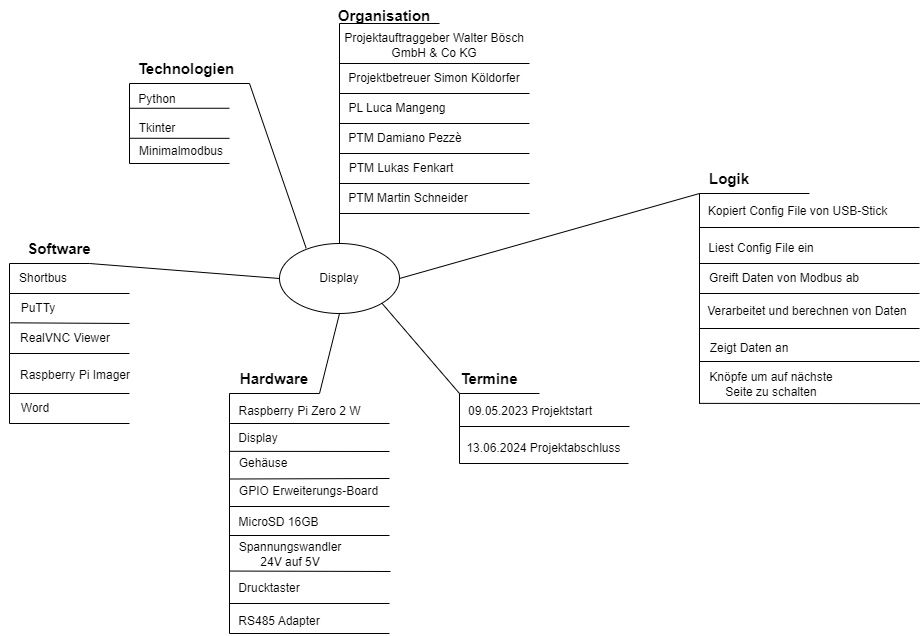
\includegraphics[width=1\linewidth]{Bilder/objektstrukturenplan}
	\caption{Objektstrukturplan}
	\label{fig:objektstrukturplan}
\end{figure}